\section{\texorpdfstring{Periferní obvody}{Periferni obvody}}

% =====================================================================================================================
	\begin{frame}
    \frametitle{MCU - jednočip}

		\textbf{CPU} - \textbf{C}entral \textbf{P}rocessing \textbf{U}nit
		
		\begin{itemize}
			\item Výpočetní jednotka (ALU),
			\item řadič instrukcí,
			\item systémové registry.
		\end{itemize}
		
		\vspace{3mm}
		\textbf{MCU} - \textbf{M}icro\textbf{c}ontroller \textbf{U}nit
		
		\begin{itemize}
			\item obsahuje vše co CPU, ale má navíc na čipu
			\item paměť RAM, FLASH,
			\item periférie jako digitální vstupy a výstupy,
			\item ADC, UART, SPI, ...
		\end{itemize}
		
	\end{frame}
	
% =====================================================================================================================
	\begin{frame}
    \frametitle{Jednočipy v porovnání s procesory}

		
		\begin{center}
			\begin{tabular}{ l | c | c }
				\hline
				\textbf{Vlastnost} & \textbf{CPU} & \textbf{MCU} \\
				\hline
				Součásti & Jen ALU & Celý systém včetně paměti \\
				Další obv. & \textbf{Ano} vždy - min. paměť & \uv{\textbf{Ne}}, kromě napájení \\
				Výkon & Vysoký & Nižší \\
				Spotřeba & Vyšší & Nižší \\
				Použití & PC, servery & \textcolor{blue}{\textbf{Embeded aplikace}} \\
				 & 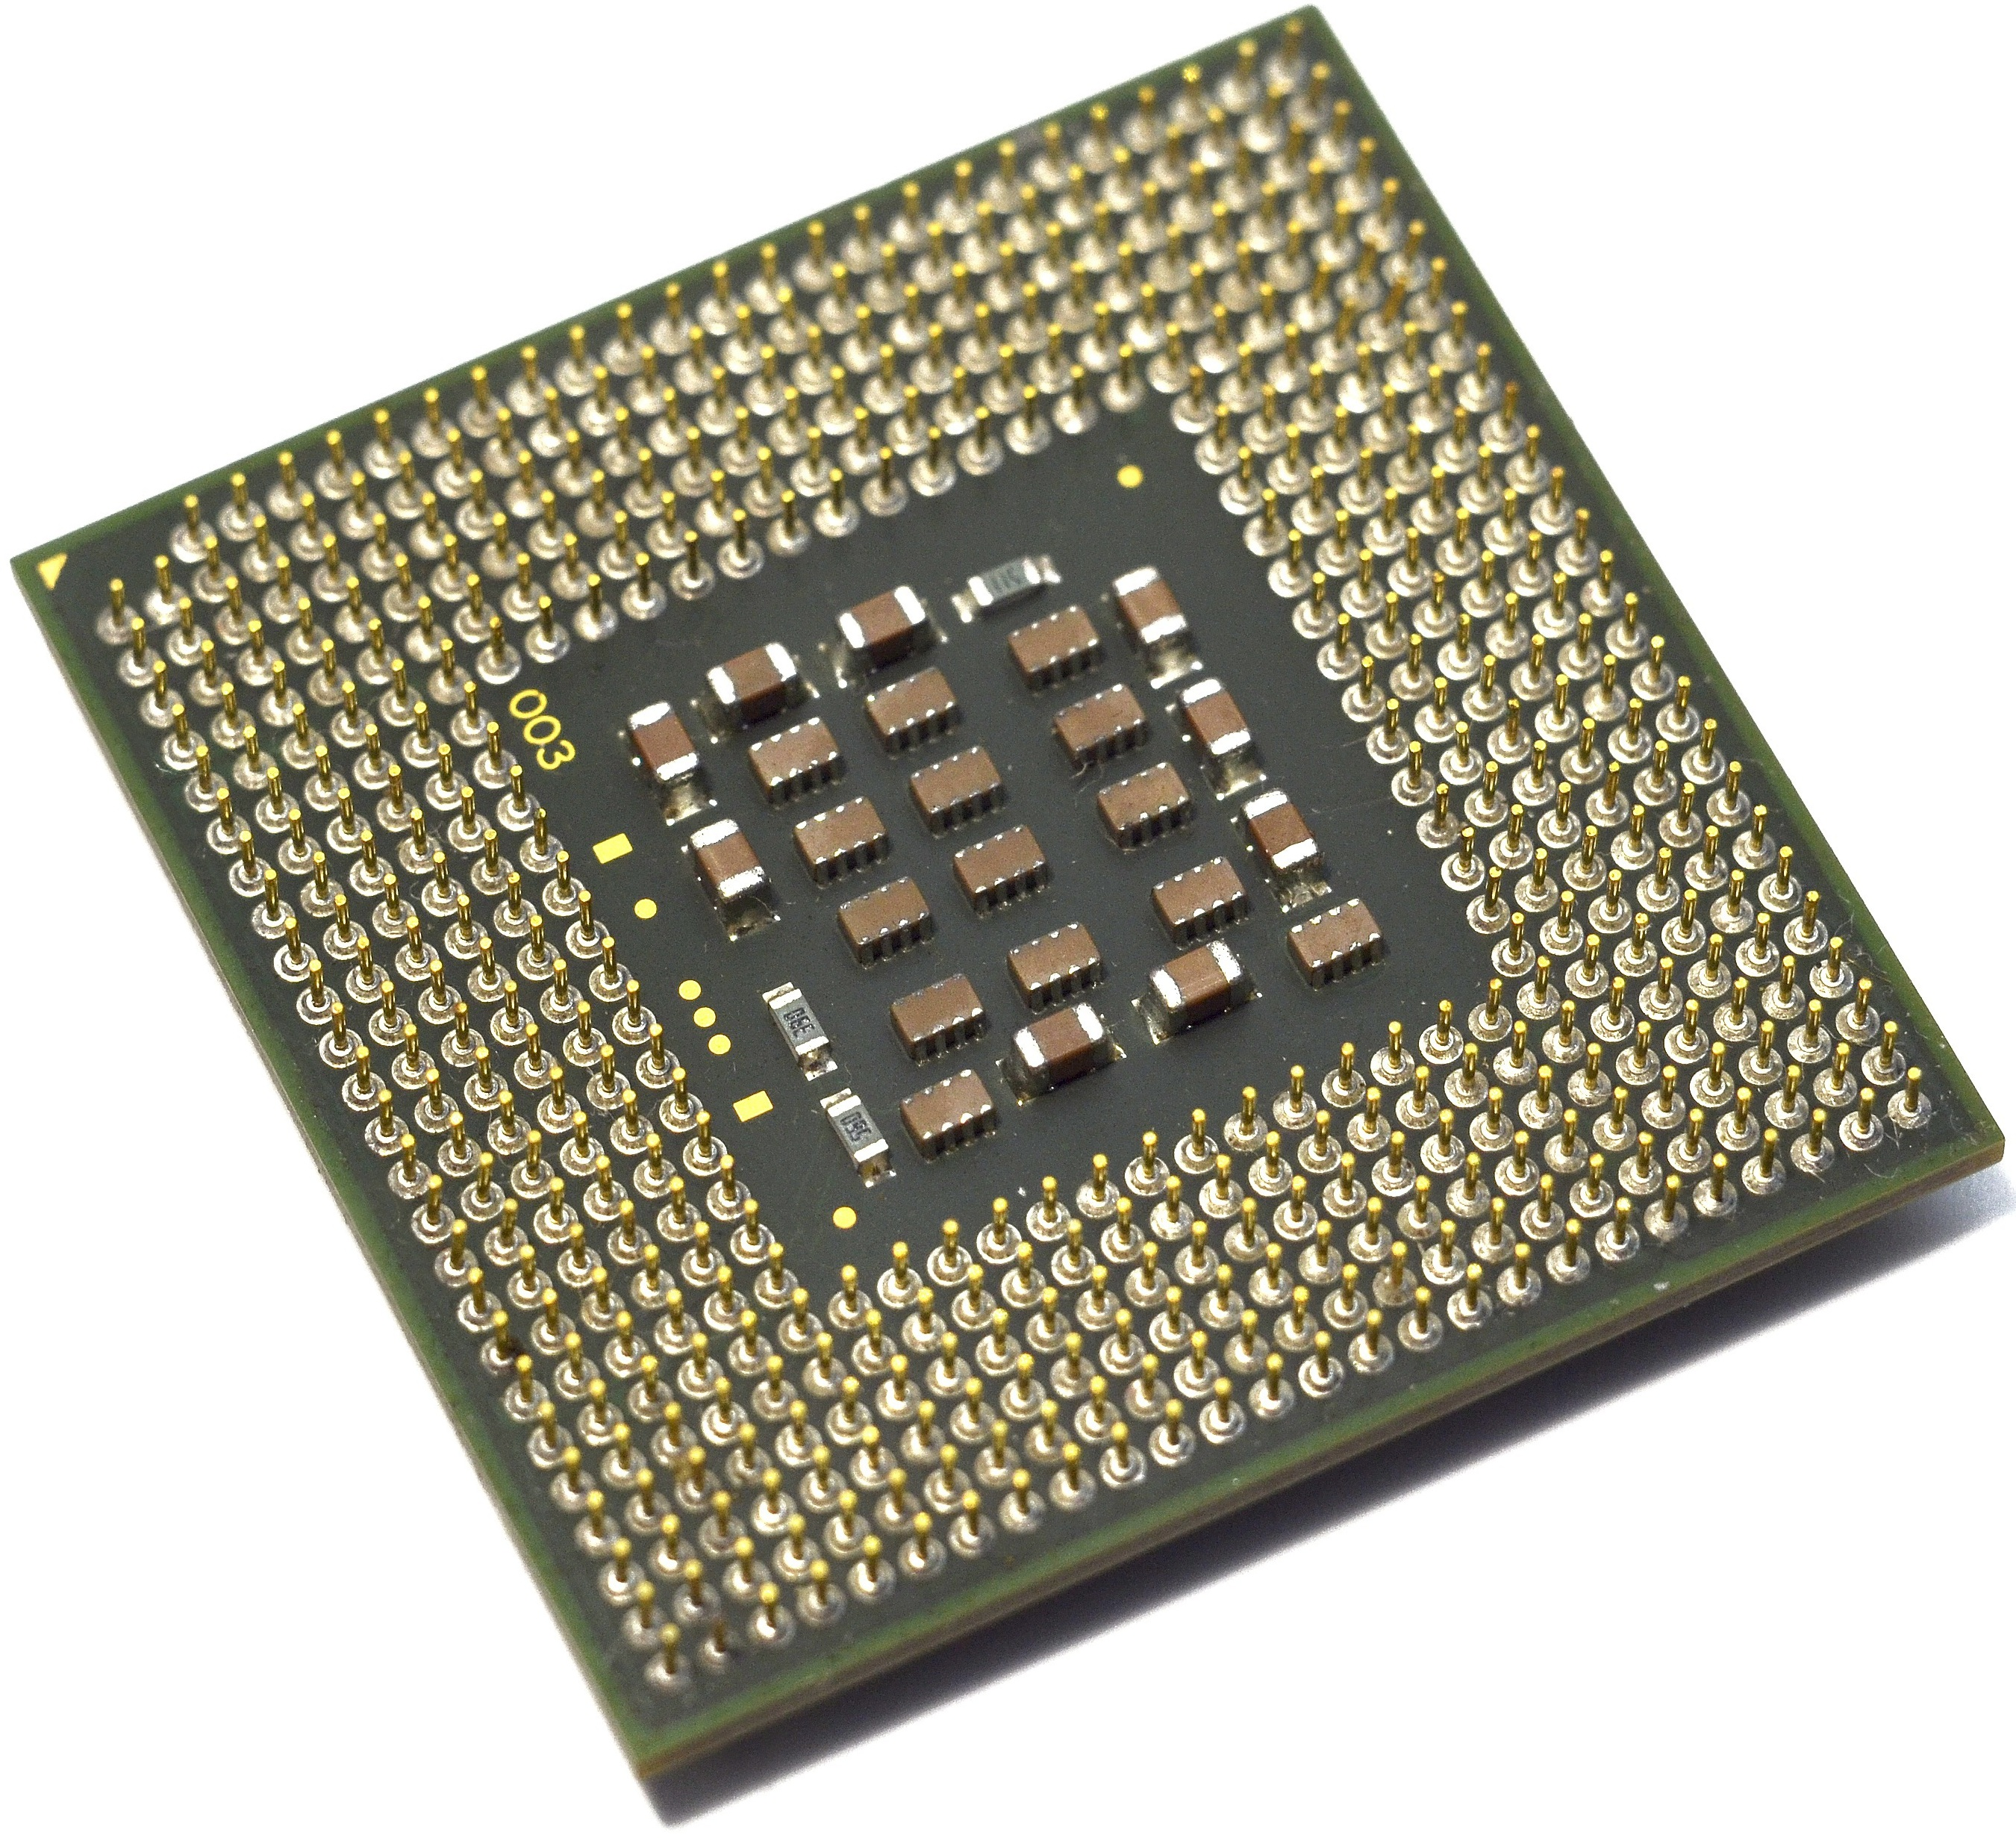
\includegraphics[width=0.25\textwidth]{fig/CPU.jpg} & 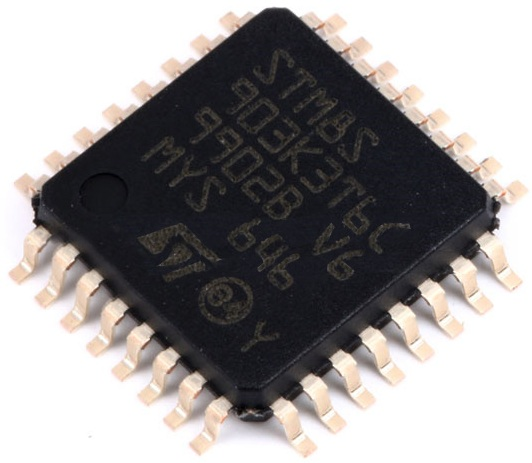
\includegraphics[width=0.25\textwidth]{fig/MCU.jpg} \\
				\hline
			\end{tabular}
		\end{center}
		
	\end{frame}
	
% =====================================================================================================================
	\begin{frame}
    \frametitle{Některé periferní obvody mcu řady STM8S}

		Konfigurace všech periférií je prováděna skrze registry:
		\vspace{3mm}
		
		\begin{itemize}
			\item Digitální vstupy a výstupy - příklad je v minulé přednášce, organizace po branách (8 pinů) PA, PB, ...
			
			\begin{itemize}
				\item \textbf{P\textcolor{blue}{[A..F]}\_CR1}... nastavení push-pull/ pull-up,
				\item \textbf{P\textcolor{blue}{[A..F]}\_DDR}... volba režimu vstupu nebo výstupu na pinu,
				\item \textbf{P\textcolor{blue}{[A..F]}\_IDR}... aktuální logická hodnota pinů (čtení),
				\item \textbf{P\textcolor{blue}{[A..F]}\_ODR}... nastavovaná logická hodnota pinů (zápis).
			\end{itemize}
			
			\vspace{3mm}
			\item ADC - analogově digitální převod, viz dále,
			\item univerzální časovač / čítač, viz dále,
			\item UART (\textbf{U}niversal \textbf{A}synchronous \textbf{R}eceiver/\textbf{T}ransmitter), sériová komunikace, nebudeme dělat.
		\end{itemize}
		
	\end{frame}